\subsection{CDC efficeicny} \label{sec:CDC_eff}
\begin{figure}[htbp]
  \begin{tabular}{ccc}
    \begin{minipage}{0.33\hsize}
      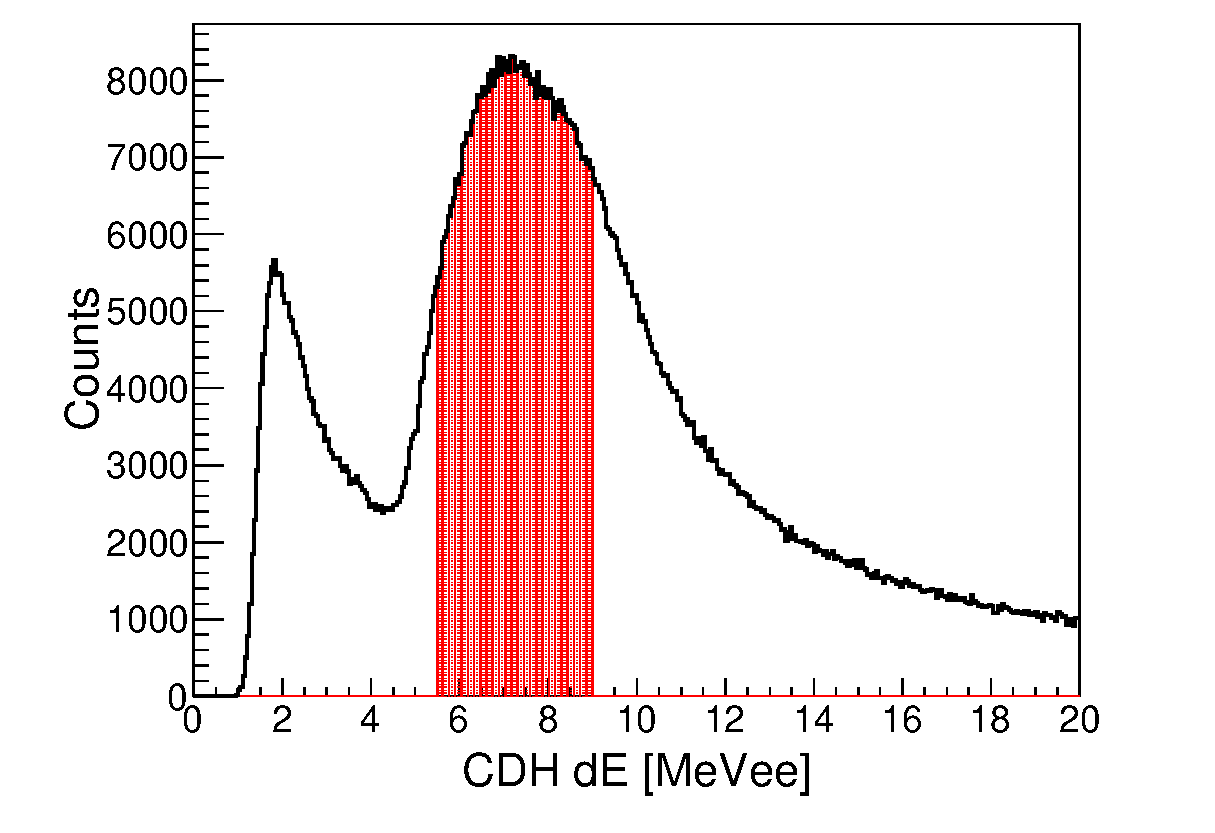
\includegraphics[width=4cm]{../pic/Run68/CDC_eff/CDH_dE.eps}
    \end{minipage}

    \begin{minipage}{0.33\hsize}
      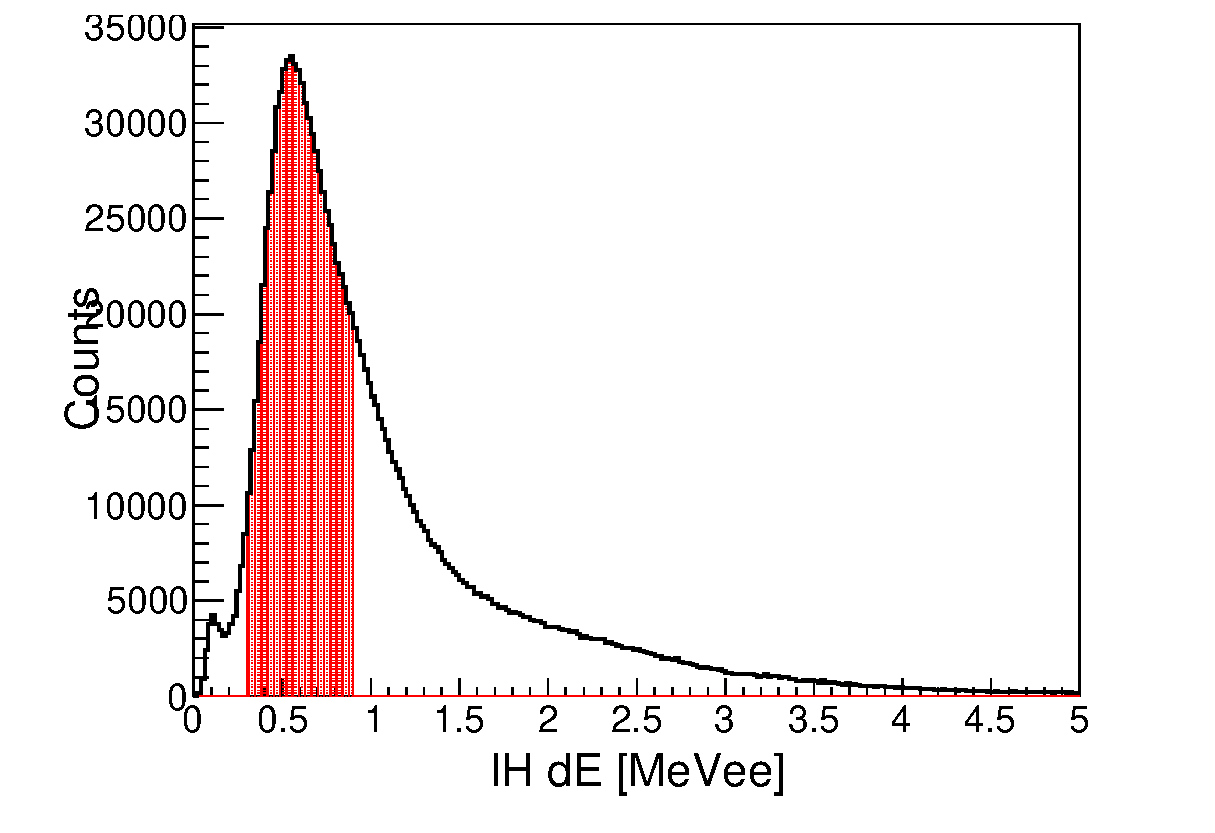
\includegraphics[width=4cm]{../pic/Run68/CDC_eff/IH_dE.eps}
    \end{minipage}
    
    \begin{minipage}{0.33\hsize}
      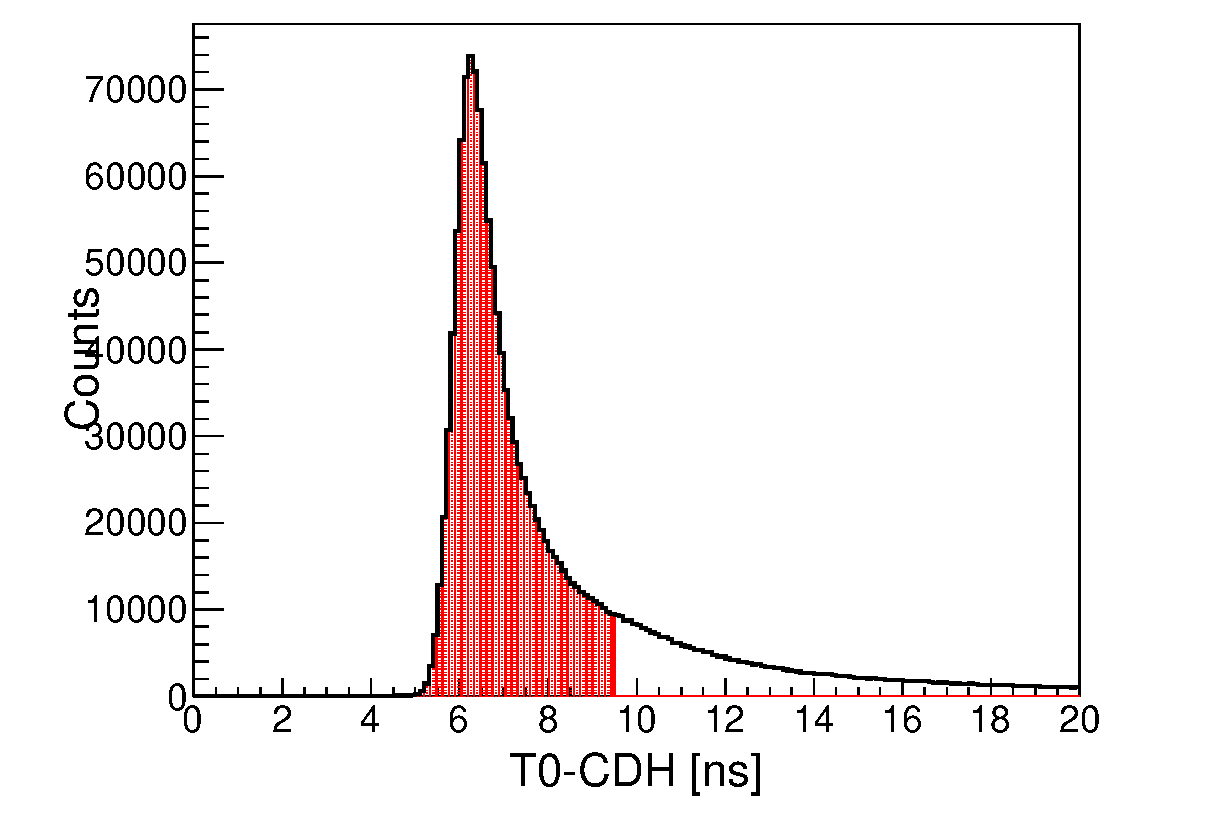
\includegraphics[width=4cm]{../pic/Run68/CDC_eff/CDH_tof.eps}
    \end{minipage}
  \end{tabular}
  \caption{
    Trigger event selection for CDC efficeincy.
    left, center and right figures show CDH dE, IH dE and T0-CDH tof.
    Red hatched region indicates acceptable region as trigger events as pass through MIP.
  }
  \label{fig:CDC_eff_trig}
\end{figure}

\begin{figure}
  \centering
  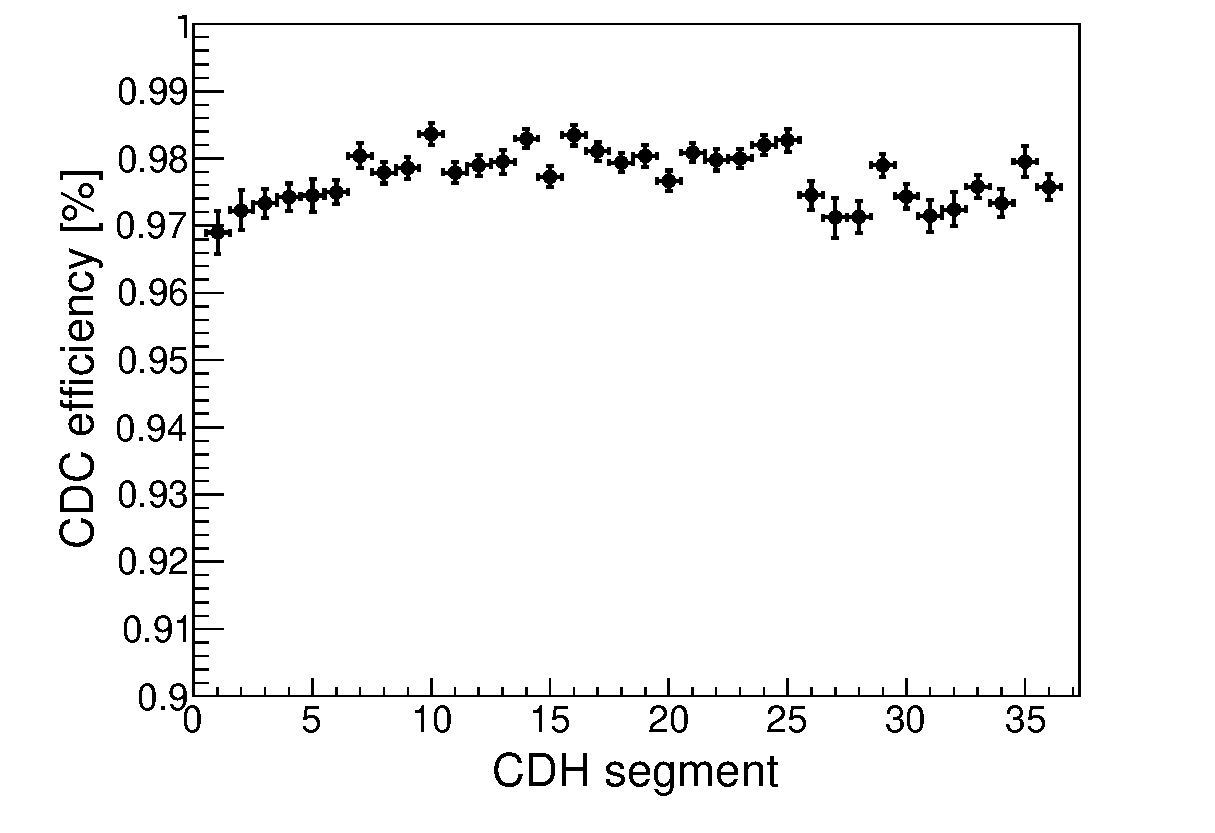
\includegraphics[width=10cm]{../pic/Run68/CDC_eff/CDC_eff_IHCDH.eps}
  \caption{
    This figure ploted CDC efficeincy about each CDH trigger segment.
  }
  \label{fig:CDC_eff}
\end{figure}

In MR-RUN69, the IH was installed at CDS which surrounding the target cell.
CDC efficiency was estimated using the IH and the CDH as trigger counter.
Trigger events was required particle like a MIP which was judged specific energy deposit at the CDH and the IH and fast timing at the CDH.
The IH do not use timing information because single read-out and bad time resolution.
The trigger event also required the CDH and The IH hit in same side which was azimuthal angle difference within 45 degree.
CDC efficiency was estimated whether can be right trajectory reconstructed.
Right trajectory was judged within a hodosocope size.
We estimated CDC efficeincy at $97.7 \pm 0.4 \%$ whose error was evaluated by fluctuation of CDH trigger segment.


